\documentclass[11pt,a4paper]{ltjsarticle}
% Compile with LuaLaTeX

\usepackage{luatexja}
\usepackage{graphicx}
\usepackage{hyperref}
\usepackage{amsmath,amssymb,mathtools}
\usepackage{xcolor}
\usepackage{float}
\usepackage{booktabs}
\usepackage{enumitem}
\usepackage{geometry}

\geometry{margin=22mm}

% =========================
% Colour scheme (WRN/rule.txt)
% =========================
\definecolor{SciBlue}{HTML}{1C3177}      % Primary
\definecolor{DeepIndigo}{HTML}{4B0082}   % Accent
\definecolor{MistLavender}{HTML}{E8EAF1} % Pale
\definecolor{MidnightInk}{HTML}{101426}  % Dark
\definecolor{OpticWhite}{HTML}{FFFFFF}   % Background

\color{MidnightInk}

\newcommand{\sectionblock}[1]{%
  \vspace{4mm}
  {\large\textbf{\textcolor{SciBlue}{#1}}}
  \vspace{2mm}

}

\newcommand{\todo}[1]{\textcolor{red}{#1}}

\title{Weekly Report (Work Plan): Acceptance Criteria for the Uncertainty Propagation}
\author{Risei Abe (Institute of Science Tokyo)}
\date{Week: 2026/09/07 -- 2026/09/14}

\begin{document}

\maketitle

% =========================================================
% 1. Question / Purpose
% =========================================================
\sectionblock{Question}

Which acceptance criteria connect the propagated kernel-extraction error, for the ladder step positions and the 5\% tolerance band, to the experimental design?

% =========================================================
% 2. Hypothesis
% =========================================================
\sectionblock{Hypothesis}

Acceptance should be defined not by the absolute wavelength endpoints but by three quantities --- the spread of the step boundaries in \emph{logarithmic power ratio}, the number of grid points required at 1\% precision, and the probability of missing a step (the previous draft compared wavelength endpoints with the dimensionless grid ratio 1.227, which is a comparison of unlike quantities and was wrong).

% =========================================================
% 3. Evidence / Interpretation
% =========================================================
\sectionblock{Evidence / Interpretation}

\begin{itemize}[leftmargin=8mm]
  \item The inputs are already fixed by the figure cross-check (E3): the sideband reproduces to within 1.0\% with \(r=1.00\) and matching peaks, while the ZPL side carries a \(\sim\)2\% read-off error on the Debye--Waller factor from the axis calibration. The ZPL peak height is unusable because of clipping.
  \item Figure~\ref{fig:ladder} shows why the criterion must be stated in log power. The quantity at risk is the position of the six vertical boundaries, and they are not equally exposed: the pair at \(1.5145\) and \(1.5191\) is separated by 0.3\% in power, so the \(N=6\) plateau between them is already unreachable before any error is added, whereas the boundaries at \(1.8646\) and \(4.2989\) stand clear by factors of 1.23 and 1.19. Whether a propagated error matters is therefore a question about spacing in \(\log I\), not about nanometres.
\end{itemize}

\begin{figure}[H]
  \centering
  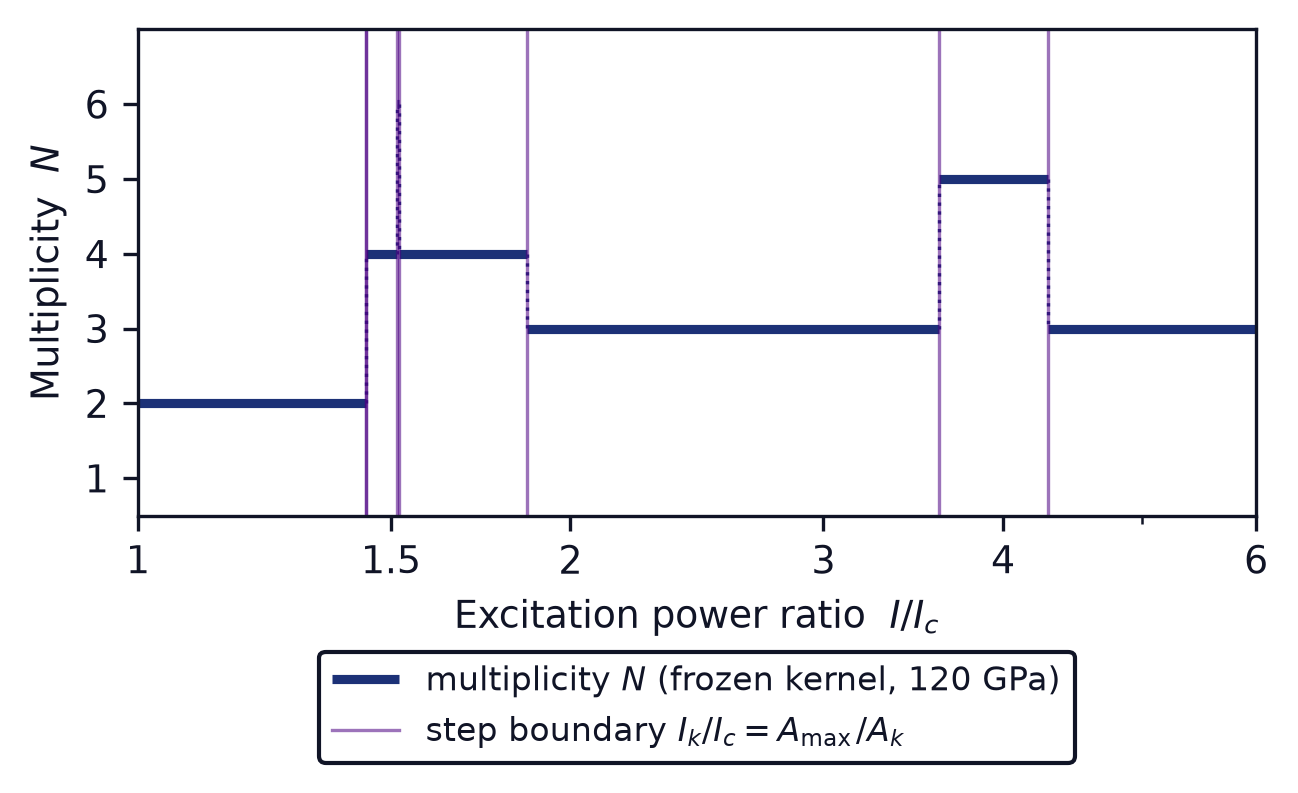
\includegraphics[width=0.58\linewidth]{image/wrn_ladder_steps.png}
  \caption{Multiplicity ladder \(N(I/I_c)\) computed from the frozen v3 kernel at
  120 GPa. Vertical lines mark the step boundaries \(I_k/I_c=A_{\max}/A_k\) at
  \(1.4414\), \(1.5145\), \(1.5191\), \(1.8646\), \(3.6079\) and \(4.2989\). The
  \(N=6\) plateau spans only 0.3\% in power and is not resolvable.}
  \label{fig:ladder}
\end{figure}

% =========================================================
% 4. Gap / Failure
% =========================================================
\sectionblock{Gap / Failure}

\begin{itemize}[leftmargin=8mm]
  \item Because the Monte Carlo has not been run, the question of whether these boundaries are stable under propagated error remains unanswered in this report; the figure shows their nominal positions only.
  \item The knobs of the v1 \texttt{default\_randomiser} are unusable, as the quantities they addressed no longer exist. The randomiser must be replaced wholesale before the propagation can start.
\end{itemize}

% =========================================================
% 5. Next Step
% =========================================================
\sectionblock{Next Step}

Implement the Monte Carlo with 1\% sideband and 2\% DWF inputs, and report its output as the three quantities: step-boundary spread in log power ratio, required number of grid points, and step-miss probability.

% =========================================================
% 6. References
% =========================================================
\sectionblock{References}

\begin{enumerate}[leftmargin=8mm]
  \item K. O. Ho, C. Dailledouze, V. \v{Z}alandauskas \textit{et al.}, ``Optical Stability and Photophysics of NV Centers in Diamond up to 120 GPa,'' arXiv:2606.02399v1 [quant-ph] (2026). Source of the optical kernel \(A(\lambda,P)\), reconstructed from Fig.~1(e).
  \item A. Dr\'eau \textit{et al.}, ``Avoiding power broadening in optically detected magnetic resonance of single NV defects for enhanced dc magnetic field sensitivity,'' \textit{Phys. Rev. B} \textbf{84}, 195204 (2011). Source of the branching exponent \(E=3\) and \(\rho^*=1/5\).
\end{enumerate}

\end{document}
